\documentclass[a4paper, 12pt,]{scrartcl}



\usepackage[utf8]{inputenc}

\usepackage[ngerman]{babel}
\usepackage{amssymb}
\usepackage[T1]{fontenc}
\usepackage{mathtools}
\usepackage{amsmath}
\usepackage{ntheorem}
\usepackage{bbm}
\usepackage{dsfont}
\usepackage{color}
\usepackage{slashed}
\usepackage{hyperref}
\usepackage{graphicx} 
\usepackage{bm}
\usepackage{mathabx}
\usepackage{float}
\usepackage{mwe}
\usepackage{changepage}
\usepackage{subcaption}
\usepackage{multirow}
\begin{document}
\begin{titlepage}
	\centering
	{\scshape\LARGE Universität Tübingen \par}
	\vspace{2cm}
	{\huge\bfseries Doppelbrechung \par}
	\vspace{2cm}
	{\Large \scshape Blockpraktikum 2021} \par
	\vspace{2cm}
	{\Large  Korrigierte Version} \par
	\vspace{2cm}
	{\Large\itshape \underline{Christian Gommeringer} \space \space  \underline{Matthias Gatter}\par}
	\vfill 
	{\large unter der Betreuung von Gina Grünauer}
	\vfill

	{\large \today\par}
\end{titlepage}
\newpage 
\tableofcontents 

\newpage
\section{Einleitung}
\begin{flushleft}
In diesem Versuch beschäftigen wir uns mit doppelbrechenden Materialien und einer ihrer Anwendungen. Zunächst wenden wir ein Verfahren zur Bestimmung der unterschiedlichen Brechungsindizes eines Materials je nach Polarisationsrichtung an. Danach untersuchen wir den Effekt der Polarisationsänderung durch sogenannte $\lambda/4$ Plättchen.


\end{flushleft}
% > < | 

\section{Theorie}
Die Theorie dieses Experiment ist leicht mit einem Grundlagenwissen in Optik zu verstehen. Es wird das Superpositionsprinzip sowie die Darstellung von ebenen Wellen durch trigonometrische Funktionen benötigt. In manchen Materialien hängt der Brechungsindex von der Polarisationsrichtung des einfallenden Lichts ab. Dies wird oft durch eine anisotrope Kristallstruktur erzeugt. Der in diesem Zusammenhang wichtige Begriff der ``optischen Achse'' bezeichnet hier eine Richtung im Medium, für die, wenn sie mit der Ausbreitungsrichtung des Lichts übereinstimmt, die Brechungsindizes unabhängig von der Polarisation sind. Wenn das Licht allerdings senkrecht zur optischen Achse einfällt, erfährt die Komponente des Lichts, die parallel zur optischen Achse polarisiert ist , einen anderen Brechungsindex als jene, die senkrecht zu ihr polarisiert ist. Durch diesen Umstand lassen sich über einen Durchgang durch dieses Medium Phasendifferenzen zwischen den beiden Polarisationsrichtungen des Lichts erzeugen.\newline\newline

Diesen Effekt nutzt der Aufbau unseres ersten Versuchs aus. Über den Durchlauf eines Materials, dessen Dicke nicht konstant ist, sondern in einer Achse durch eine Schräge leicht zunimmt. Dadurch unterscheidet sich die Phasendifferenz der beiden Komponenten des einfallenden Licht kontinuierlich vom Ort, an dem es auf die Platte trifft. Beträgt diese Phasendifferenz gerade $2\pi$, ist das austretende Licht exakt in die selbe Richtung polarisiert, wie das einfallende, ansonsten ändert es seine Polarisationsrichtung. Führt man nun vor und hinter dem Mediumblock zwei Polarisationsfilter in der optischen Bank ein, deren Richtung übereinstimmen, dann kommt um verschiedene Austrittspunkte aus dem Medium herum kein oder nur sehr wenig Licht durch den zweiten Polarisationsfilter. Nämlich gerade dort wo der Phasendifferenz gerade ungefähr $2\pi$ ist. Dort ist die Polarisation nämlich nicht verändert worden.\newline
Aus der Dickeänderung des Mediums und dem Abstand der Intensitätsminima lässt sich der Unterschied in der Brechungsindizes berechnen.
\begin{figure}[H]\centering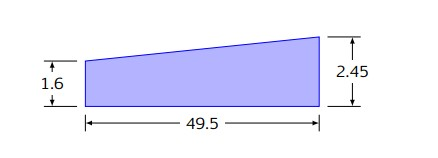
\includegraphics[scale=0.7]{Keil}\caption{Abmessungen des Quarzkeils, entnommen aus der Versuchsanleitung}\end{figure}
Es treffen ebene Wellen auf die Oberfläche des Mediums. Die auch nach Wiederaustritt aus dem Medium ihre Form von Ebenen Wellen beibehalten. Deshalb entspricht ein Abstand $l$ zwischen zwei Minima einem Dickeunterschied $\Delta{d}$ von
\begin{equation*}\Delta{d}=\frac{l}{\cos\alpha}\,c\end{equation*}
wobei $c$ die Skala der Dickeänderung bezeichnet $c=\frac{2.45-1.6}{49.5}=0.0172$. $\alpha$ ist der Winkel zwischen in das Medium eintretender und austretender Welle. Da die Dickenänderung allerdings nur sehr gering ist setzen wir $\alpha\approx0$. Daraus ergibt sich eine Phasendifferenz von
\begin{equation*}\Delta\varphi=\Delta{k}\,\Delta{d}=\Delta{n}\,k_0\,\delta{d}=\Delta{n}\,\frac{2\pi}{\lambda}\,c\,l\end{equation*}
und da diese Phasendifferenz zwischen zwei Intensitätsminima gerade $2\pi$ ist, berechnet sich daraus der Unterschied in den Brechungsindizes als
\begin{equation*}\Delta{n}=\frac{\lambda}{c\,l}\end{equation*}

Im nächsten Versuch wollen wir die Wirkung eines $\lambda/4$ Plättchens auf die Polarisierung behandeln. Dieses erzeugt eine Differenz im optischen Weg der beiden Komponenten des elektromagnetischen Felds der elektromagnetischen Welle parallel und senkrecht zur optischen Achse von eben $\lambda/4$ und damit eine Phasendifferenz von $\pi/2$. Wenn $A_1$ die Amplitude des E-Felds parallel zur optischen Achse, die wir mit der x-Achse identifizieren, ist und $A_2$ die senkrechte Komponente dann hat das E-Feld nach Durchgang durch das Plättchen die Gestalt
\begin{equation*}\vec{E}=\left(\begin{array}{c}A_1\,\cos(k\,z-\omega{t})\\A_2\,\sin(k\,z-\omega{t})\end{array}\right)\end{equation*}
Und wenn das $\lambda/4$ Plättchen nicht perfekt auf die Wellenlänge eingestellt ist, dann stellt sich noch eine zusätzliche Phasendifferenz  von $\Delta\phi$ ein, die so klein sein soll, dass man die trigonometrischen Funktionen mit erster Ordnung Taylor Approximation nähern kann. Das E-Feld hat dann die Gestalt
\begin{align*}\vec{E}&=\left(\begin{array}{c}A_1\,\cos(k\,z-\omega{t}+\Delta\phi)\\A_2\,\sin(k\,z-\omega{t})\end{array}\right)\\
&=\left(\begin{array}{c}A_1\,\left(\cos(k\,z-\omega{t})-\sin(k\,z-\omega{t})\,\Delta\phi\right)\\A_2\,\sin(k\,z-\omega{t})\end{array}\right)
\end{align*}
Projektiert auf einen bestimmten Winkel $\beta$ zur optischen Achse ist der Betrag des elektrischen Felds
\begin{align*}E(\beta)&=\left(\begin{array}{c}A_1\,\left(\cos(k\,z-\omega{t})-\sin(k\,z-\omega{t})\,\Delta\phi\right)\\A_2\,\sin(k\,z-\omega{t})\end{array}\right)\cdot\left(\begin{array}{c}\cos\beta\\\sin\beta\end{array}\right)\\
&=A_1\,\cos\beta\,\left(\cos(k\,z-\omega{t})-\sin(k\,z-\omega{t})\,\Delta\phi\right)+A_2\,\sin\beta\,\sin(k\,z-\omega{t})
\end{align*}
Daraus ergibt sich die Intensität unter Fortführung der Kleinwinkelnäherung
\begin{align*}I(\beta)=&c\,\epsilon_0\,E(\beta)^2\\
=&c\epsilon_0\,\left[A_1^2\,\cos^2\beta\,\left(\cos^2(k\,z-\omega{t})-2\,\cos(k\,z-\omega{t})\,\sin(k\,z-\omega{t})\,\Delta\phi\right)+A_2^2\,\sin^2\beta\,\sin^2(k\,z-\omega{t})\right]\\
&-c\,\epsilon_0\,A_1\,A_2\,\sin\beta\,\cos\beta\,\sin(k\,z-\omega{t})\,\left(\cos(k\,z-\omega{t})-\sin(k\,z-\omega{t})\,\Delta\phi\right)\end{align*}
Nach zeitlicher Mittelung erhält man
\begin{equation*}\langle{I(\beta)}\rangle=\frac{1}{2}\,A_1^2\,\cos^2\beta+\frac{1}{2}\,A_2^2\,\sin^2\beta-A_1\,A_2\cos\beta\,\sin\beta\,\Delta\phi\end{equation*}
Wenn man nun berücksichtigt, dass das Licht mit einer E-Feld Amplitude von $E_0$ und einem Winkel zur optischen Achse von $\alpha$ auf das $\lambda/4$ Plättchen trifft, werden die Startamplituden umgeschrieben zu $A_1=E_0\,\cos\alpha$ und $A_2=E_0\,\sin\alpha$. Das endgültige Resultat für die Intensität betragt damit
\begin{equation*}\langle{I}(\alpha,\beta)\rangle=c\,\epsilon_0\,E_0\,\left(\frac{1}{2}\,\cos^2\alpha\,\cos^2\beta+\frac{1}{2}\,\sin^2\alpha\,\sin^2\beta-\cos\alpha\,\cos\beta\,\sin\alpha\,\sin\beta\,\Delta\phi\right)\end{equation*}


\section{Versuchsdurchführung}
Für den ersten Versuch zur Bestimmung der Differenz der Brechungsindizes verwendeten wir folgenden Aufbau.
\begin{figure}[H]\centering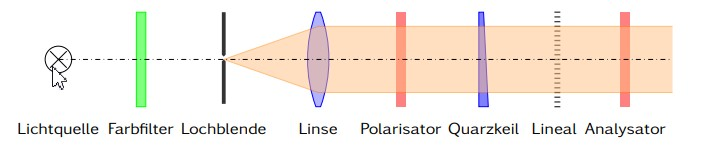
\includegraphics[scale=0.8]{Aufbau V1}\caption{Versuchsaufbau zur Messung der Brechungsindizes; entnommen aus der Versuchsanleitung}\end{figure}
Wie zu sehen ist, wird das Lichtbündel nach Durchgang durch den Farbfilter so präpariert, dass es in parallelen Strahlen auf die Oberfläche des Mediums trifft. Das Medium besteht hier aus Quarz. Polarisator und Analysator sind wie oben beschrieben auf die selbe Richtung eingestellt und es werden mit Hilfe des Lineals die Abstände der Minima gemessen. Wir maßen dazu den Abstand von entfernten Intensitätsminima um den Messfehler zu reduzieren. Unsere Messwerte sind in folgender Tabelle dargestellt.
\begin{table}[H]\centering\begin{tabular}{c  |c  |c |c }Wellenlänge&435.8 nm (blau)&546.3 nm (grün)&578 nm (gelb)\\\hline\multirow{3}{3cm}{Abstand zwischen zwei Minima in cm}&0,25&0,3167&0,37\\&0,2556&0,3375&0,3667\\&0,2563&0,3429&0,35\end{tabular}\caption{Messergebnisse aus Versuch 1}\end{table}
Für den zweiten Teil des Versuchs verwendeten wir folgenden Aufbau
\begin{figure}[H]\centering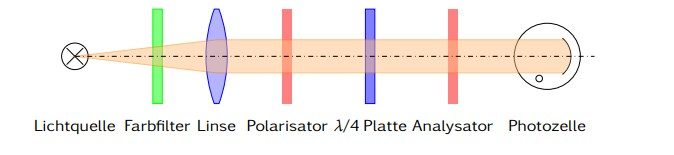
\includegraphics[scale=0.8]{Aufbau V2}\caption{Versuchsaufbau zum Experiment mit dem 
$\lambda/4$ Plättchen, entnommen aus der Versuchsanleitung}\end{figure}
Hierbei maßen wir für Polarisatorstellungen von 0°, 15°,30° und 45° (gemessen jeweils zur Achse senkrecht zum Tisch) die Intensität die in der Fotozelle registriert wurde in Abhängigkeit zur Analysatorstellung, die wir in 15° Schritten veränderten.

\section{Auswertung}
Aus den Messdaten ließen sich die Differenzen in den Brechungsindizes in Abhängigkeit von der Wellenlänge mit der in der Theorie abgeleiteten Formel berechnen
\begin{align*}\Delta{n_b}&=0.01\pm2.7\cdot10^{-4}\,(\text{stat.})\pm0.00395\,(\text{sys.})\\
\Delta{n_{gr}}&=0.00957\pm7.97\cdot10^{-4}\,(\text{stat.})\pm0.00289\,(\text{sys.})\\
\Delta{n_{gl}}&=0.00929\pm5.5\cdot10^{-4}\,(\text{stat.})\pm0.00257\,(\text{sys.})\end{align*}
Der statistische Fehler wird im gesamten Protokoll über das Gaußsche Fehlerfort, systematischer Fehler über den Betrag der Komponenten aus 1. Taylor Approximation. Außerdem nahmen wir als systematischen Fehler die Hälfte der kleinsten Ableseeinheit plus 0.5 Promille des Messwertes.\newline
Während der Versuchsdurchführung nahmen wir den Effekt wahr, dass es vier Einstellungen des Polarisators gab, bei dem bei keiner Analysatorstellung ein Streifenmuster zu beobachten war. Dies lässt sich damit erklären, dass diese Stellungen gerade eine Position senkrecht oder parallel zur optischen Achse trafen, und es daher keinen Unterschied im Brechungsindex zwischen zwei Komponenten des Lichts gab.\newline\newline

Für den zweiten Versuchsteil bestimmten wir die Intensität des Elektrischen Felds des Lichts in Abhängigkeit vom Winkel in der Ebene senkrecht zur Ausbreitung, bei verschiedenen Polarisator Einstellungen. Dazu maßen wir die Spannung, die die Fotozelle ausgab, welche proportional zur gesuchten Intensität ist.

\begin{table}[H]\centering\begin{tabular}{c |ccc}Winkel $\beta$ in °&\multicolumn{3}{c}{Spannung in V}\\\hline
0	&110	&125	&157\\
15&	420	&475	&455\\
30	&610	&614	&614\\
45&	640	&635	&639\\
60	&650	&650	&650\\
75	&657	&658	&658\\
90	&658	&659	&659\\
105	&654	&653	&654\\
120	&648	&644	&645\\
135	&632	&626	&629\\
150	&596	&588	&594\\
165	&299	&295&	294\\
180	&350&	97&	113\end{tabular}\caption{Messwerte für den Zyklus Polarisatorstellung 0°, die Stellung des Analysators ist immer auf einen unbekannten Nullpunkt der Winkelskala bezogen, was keine Auswirkung auf die Auswertung der Daten hat.}\end{table}



\begin{table}[H]\centering\begin{tabular}{c |ccc}Winkel $\beta$ in °&\multicolumn{3}{c}{Spannung in mV}\\\hline
0&	557	&555	&565\\
15&	599	&598	&604\\
30	&622	&623	&623\\
45	&640	&640	&639\\
60	&649	&649	&649\\
75	&654	&654	&653\\
90	&653	&653	&654\\
105	&649	&650	&650\\
120	&642	&643	&642\\
135	&626&626	&628\\
150	&602	&610	&608\\
165	&548	&577	&574\\
180	&531	&553	&542
\end{tabular}\caption{Messwerte für den Zyklus Polarisatorstellung 15°, die Stellung des Analysators ist immer auf einen unbekannten Nullpunkt der Winkelskala bezogen, was keine Auswirkung auf die Auswertung der Daten hat.}\end{table}



\begin{table}[H]\centering\begin{tabular}{c |ccc}Winkel $\beta$ in °&\multicolumn{3}{c}{Spannung in mV}\\\hline
0	&621	&621	&621\\
15	&626	&627	&626\\
30	&633	&634	&634\\
45	&639	&639	&639\\
60	&643	&642	&643\\
75&	644	&644	&644\\
90	&642	&642	&642\\
105	&639	&639	&639\\
120	&633	&633	&634\\
135	&627	&627	&626\\
150	&622	&622	&621\\
165	&618&	618	&618\\
180	&620	&620	&620    
\end{tabular}\caption{Messwerte für den Zyklus Polarisatorstellung 30°, die Stellung des Analysators ist immer auf einen unbekannten Nullpunkt der Winkelskala bezogen, was keine Auswirkung auf die Auswertung der Daten hat.}\end{table}

\begin{table}[H]\centering\begin{tabular}{c |ccc}Winkel $\beta$ in °&\multicolumn{3}{c}{Spannung in mV}\\\hline
0	&643&	643	&643\\
15	&643&	643	&643\\
30	&641&	641	&641\\
45	&636&	637	&637\\
60	&630&	631	&631\\
75	&624&	624	&624\\
90	&620&	621	&620\\
105	&619&	620	&620\\
120	&623&	623	&623\\
135	&628	&629	&629\\
150	&635	&636	&635\\
165	&640	&640	&640\\
180	&643	&643&	642
\end{tabular}\caption{Messwerte für den Zyklus Polarisatorstellung 45°, die Stellung des Analysators ist immer auf einen unbekannten Nullpunkt der Winkelskala bezogen, was keine Auswirkung auf die Auswertung der Daten hat.}\end{table}

Wir führten für jedes Winkelpaar drei Messungen durch, um Auswirkungen von Schwankungen in der Lichtquelle zu reduzieren. Zur Auswertung normierten wir die Messwerte auf den maximalen Wert aller Messpunkte. Anschließend können wir unsere Messung in einem Polardiagramm darstellen. Wir spiegelten für eine bessere Anschauung dazu unsere Messwerte am Ursprung.
\begin{figure}[H]\centering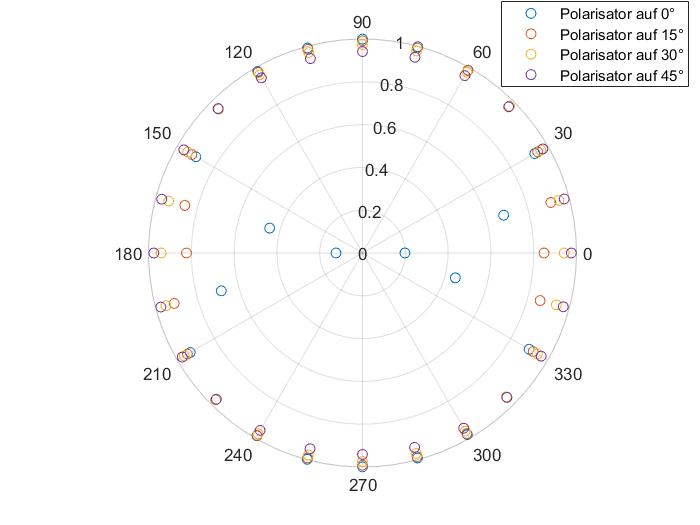
\includegraphics[scale=0.5]{tot2}\caption{Darstellung der Messwerte im Polardiagramm. Es muss beachtet werden, dass die Kurven gegebenenfalls gegen einander gedreht werden müssen, um den Zusammenhang korrekt darzustellen.}\end{figure}

%\begin{figure}[H]\centering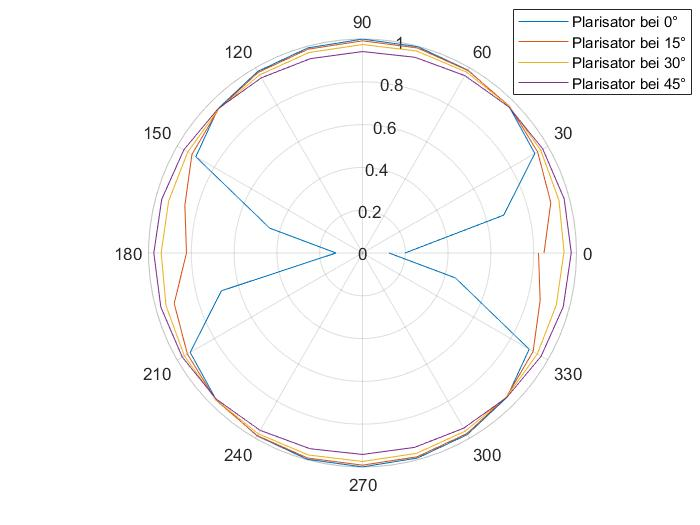
\includegraphics[scale=0.5]{totpolarplot}\caption{Nochmal das selbe wie oben, nur mit Verbindungslinien zwischen den Messpunkten, damit die Form besser erkannt werden kann. Es muss betont werden, dass die Linien nicht gemessen wurden und daher für die physikalische Interpretation nicht berücksichtigt werden dürfen. Ich halte es aber für interessant, welche Form sich ergeben würde, wenn man die Punkte mit einander verbände.}\end{figure}


\begin{figure}[H]\centering
\begin{adjustwidth}{-1em}{7em}
  \begin{subfigure}[b]{0.5\textwidth}
    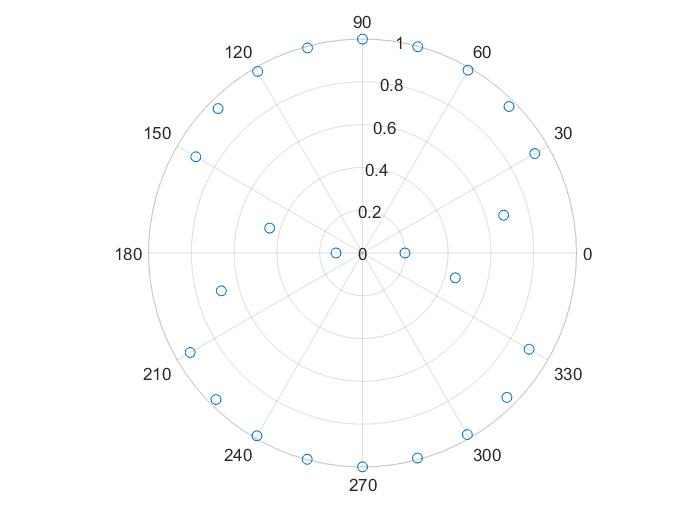
\includegraphics[width=\textwidth]{M1}
    \caption{Polarisator 0°}
    \label{fig:}
  \end{subfigure}
  %
  \begin{subfigure}[b]{0.5\textwidth}
    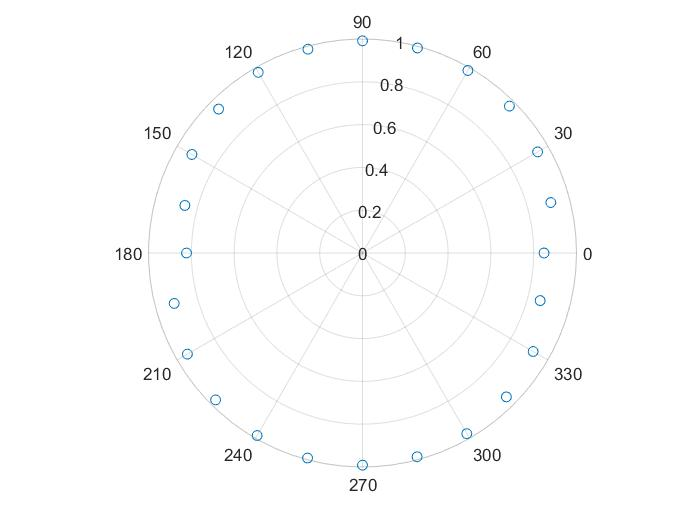
\includegraphics[width=\textwidth]{M2}
    \caption{Polarisator 15°}
    \label{fig:}
  \end{subfigure}
\end{adjustwidth}\centering
\begin{adjustwidth}{-1em}{7em}
  \begin{subfigure}[b]{0.5\textwidth}
    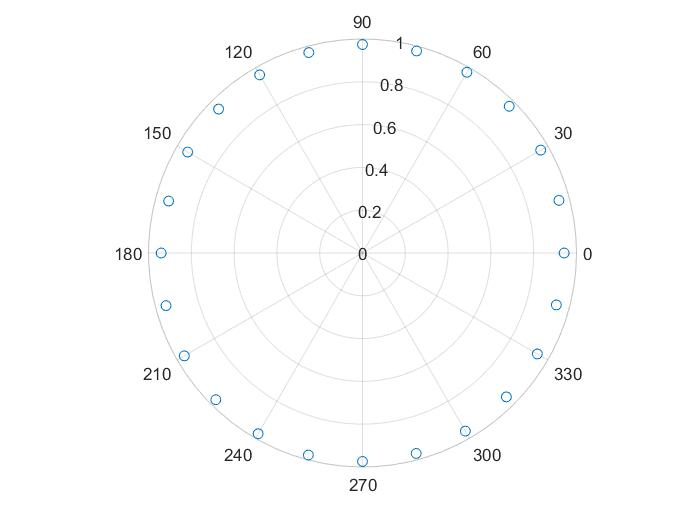
\includegraphics[width=\textwidth]{M3}
    \caption{Polarisator 30°}
    \label{fig:}
  \end{subfigure}
  %
  \begin{subfigure}[b]{0.5\textwidth}
    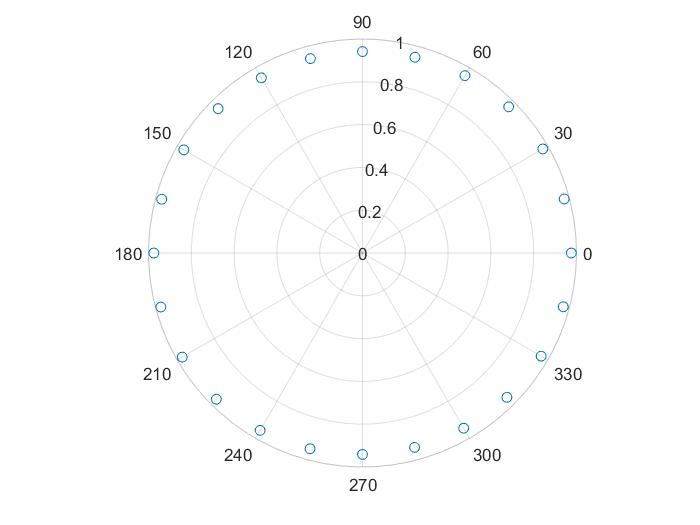
\includegraphics[width=\textwidth]{M4}
    \caption{Polarisator 45°}
    \label{fig:}
  \end{subfigure}
\end{adjustwidth}
\caption{nochmalige Gegenüberstellung der Messergebnisse. Als Betrag ist jeweils die auf das globale Maximum normierte Spannung Aufgetragen}
\end{figure}
 Zum Schluss möchten wir noch untersuchen, wie gut die Messwerte mit unserer Erwartung aus der Theorie übereinstimmen. Dazu passten wir an die Daten eine Funktion der Form $$f=a_1\,\left(\cos^2(a_2)\,\cos^2(\beta-a_3)+\sin^2(a_2)\,\sin^2(\beta-a_3)-2\,\cos(a_2)\,\sin(a_2)\,\cos(\beta-a_3)\,\sin(\beta-a_3)\,a_4\right)$$
an. Die Ergebnisse sind in folgender Tabelle zusammengefasst.
\begin{table}[H]\centering\begin{tabular}{|c |c |c |c |c |}\hline{Polarisatoreinstellung}&$a_1$&$a_2$&$a_3$&$a_4$\\\hline
0°&3.2275&2.1576&-0.0986&-0.0505\\\hline
15°&3.762&2.3444&0.5335&0.0716\\\hline
30°&3.8372&2.3556&0.4986&0.02\\\hline
45°&3.8356&2.3653&0.0424&0.0046\\\hline\end{tabular}\caption{Regressionsparameter für die verschiedenen Anpassungen}\end{table}

\begin{figure}[H]\centering
\begin{adjustwidth}{-1em}{7em}
  \begin{subfigure}[b]{0.5\textwidth}
    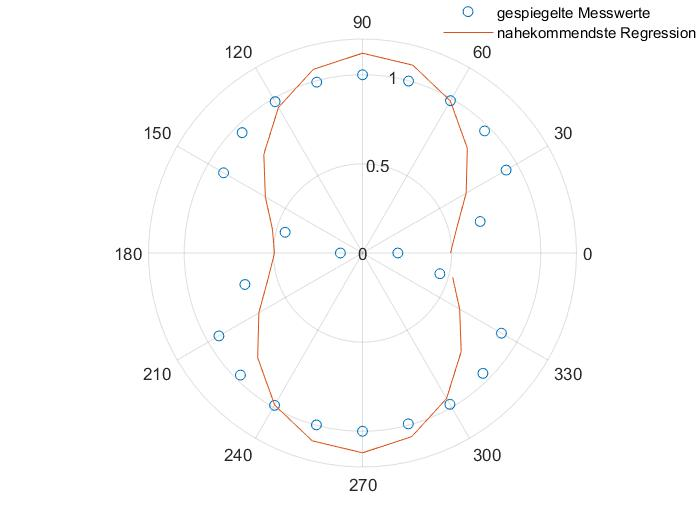
\includegraphics[width=\textwidth]{Fit1}
    \caption{Polarisator 0°}
    \label{fig:}
  \end{subfigure}
  %
  \begin{subfigure}[b]{0.5\textwidth}
    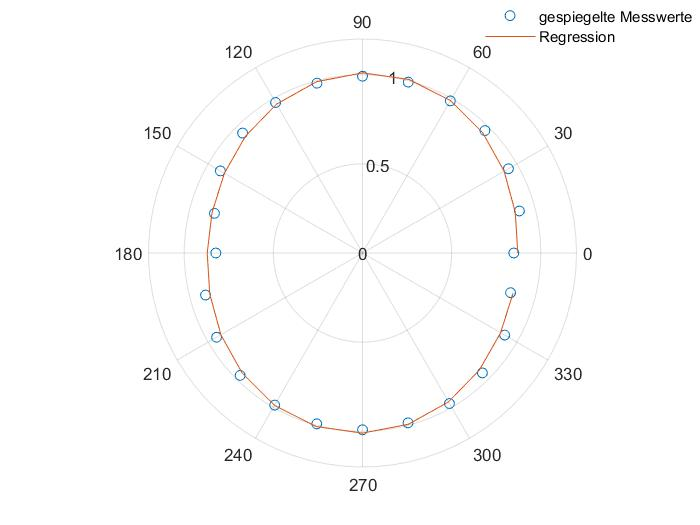
\includegraphics[width=\textwidth]{Fit2}
    \caption{Polarisator 15°}
    \label{fig:}
  \end{subfigure}
\end{adjustwidth}\centering
\begin{adjustwidth}{-1em}{7em}
  \begin{subfigure}[b]{0.5\textwidth}
    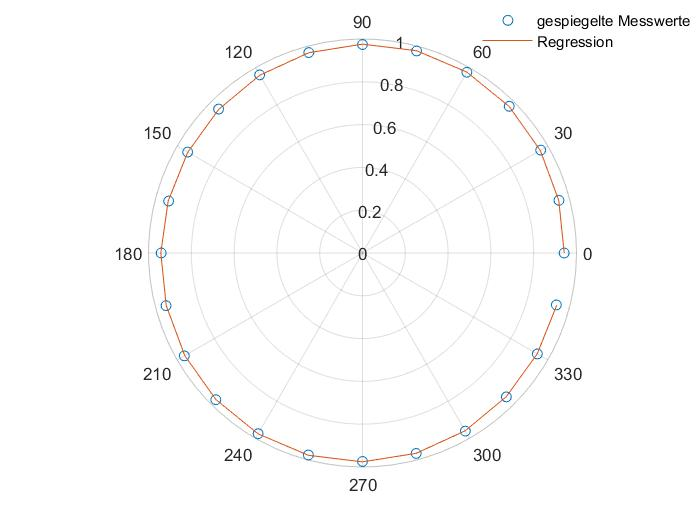
\includegraphics[width=\textwidth]{Fit3}
    \caption{Polarisator 30°}
    \label{fig:}
  \end{subfigure}
  %
  \begin{subfigure}[b]{0.5\textwidth}
    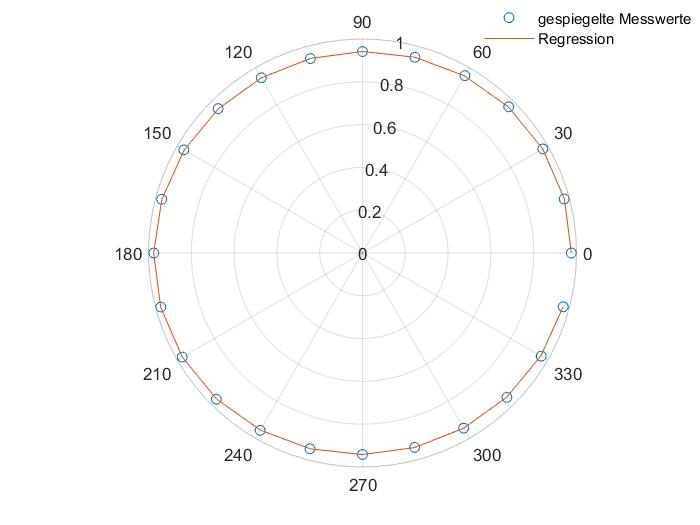
\includegraphics[width=\textwidth]{Fit4}
    \caption{Polarisator 45°}
    \label{fig:}
  \end{subfigure}
\end{adjustwidth}
\caption{gespiegelte Messdaten zusammen mit den Fits}
\end{figure}

Es ist deutlich zu erkennen, dass die Regression für den ersten Fall überhaupt nicht passt. Das deutet darauf hin, dass wir in unserem Modell einen Effekt nicht berücksichtigt habe, der in diesem Fall aber von Bedeutung ist. Für die Polarisatorstellung ``0°'' gibt es ein ausgeprägtes Minimum, wo die Intensität fast verschwindet. Es ist daher anzunehmen, dass die der Polarisator in der Tat das Licht in eine Richtung polarisiert, die parallel oder senkrecht zur optischen Achse des Mediums liegt. In diesem Fall müsste die Intensität ungefähr der Form $I(\beta)\approx{a_1}\,\sin^2(\beta)$ folgen. Es ist aber erkennbar, dass die gemessene Kurvenform einfach nicht mir diesem Ergebnis übereinstimmt, da sie viel zu abrupt abfällt und davor zu konstant ist. Möglicherweise ist die Messkurve noch durch unerwünschtes gestreutes Licht verfälscht worden.

\section{Fazit}
Mit unseren Ergebnissen für die Differenz im Brechungsindex von Quarz sind wir zufrieden. Das Lexikon der Physik von spektrum.de gibt die Differenz für Quarz bei Licht der Wellenlänge 589,3 nm zu 0,0091 an. Damit wirken unsere Resultate plausibel. Bis auf die erste Messung konnten auch an die Messdaten des zweiten Versuchs gut die theoretische Erwartung angepasst werden. Die Messwerte der Messungen 2-4 bei Versuch zwei stimmen sehr gut mit der theoretischen Erwartung überein, wie den Schaubildern zu entnehmen ist. Das Scheitern bei der ersten Messung kann wahrscheinlich auch auf Schwächen im Versuchsaufbau, wie Verschmutzung der Messung durch Restlicht im Raum, zurückgeführt werden. 














\end{document}